\section{Experimentación}
En esa sección, para entender las causas y consecuencias de OTP, se plantean dos ejes de experimentación.
\subsection{Primer eje de experimentación}
% OTP como kpi, como es importante queremos ver si es predecible
% la necesidad de entenderlo en que situaciones es mas o menos confiable:
En el primer eje intentaremos analizar a OTP como KPI, es decir qué tan bien evalúa la calidad de los factores involucrados en el transporte aéreo y qué tipo de consideraciones hay que tener sobre su naturaleza para usarla como herramienta predictiva de rendimiento.

% recorte de outliers: por que?
Usaremos el promedio de delay por unidad de tiempo, de modo de ajustar por cantidad de vuelos nuestras predicciones, y también contrastaremos la diferencia entre considerar datos con outliers y considerarlos en crudo en términos cuál brinda mejor calidad predictiva.

\subsubsection{Estacionalidad}
% hablar de estacionalidad y senos (fases, por que no usamos cosenos):
%             como evoluciona la metrica con el tiempo
% que fases nos interesan y por que (overfitting, verano yankee, etc)
% como esperamos que sean los coeficientes de las fases (en las vacaciones grandes, durante el año mal)
% que granularidad anduvo mejor, anduvo mejor con o sin outliers? por que?
% que pinta tiene la curva final
%hablar matrices singulares ec normales por el tema de fases
Lo primero que intentamos analizar es la variación estacional de las métricas: la congestión aeroportaria dificilmente sea constante a lo largo del año sino que es de esperarse que en épocas del hemisferio norte como vaciones de invierno, verano y primavera aumente.

Interesantemente tuvimos en varios casos mejores resultados sin recortar \footnote{Se recorta el 10\% de los menores y mayores retrasos} outliers para el promedio de delays por dia o meses. En general la granularidad diaria funcionó mejor que la mensual para predicciones: se esperaría que la congestión crezca los fines de semana, información que se pierde mensualmente. Obtuvimos los menores errores de predicción en las particiones más cercanas al 50/50, lo que tiene sentido en términos de underfitting y overfitting. Para el caso diario conseguimos el NRMSE de predicción mínimo al rededor de 0.09 con coeficientes de frecuencias mayores principalmente semanales, trimestrales, semestrales y anuales (en orden descendente) y en $\frac{2}{5}$ del dataset para entrenamiento y el resto de predicción, mientras que con $\frac{1}{5}$ para entrenamiento se consiguió el peor a pesar de que fitteaba mejor sobre el set de training.


\subsubsection{OTP como KPI para aeropuertos, aerolíneas y rutas aéreas}
% mejor como kpi de aeropuertos vs aerolíneas vs rutas aereas?
% que creeria uno?
% por que top 5
% boxplot (como se consigue), por que tiene sentido y que dice de la correlacion entre categorias
Luego nos planteamos cómo influye cada factor en el delay, y por consiguiente sobre qué factor es mejor KPI el OTP. Comparamos predicciones mensuales del top 5 en volumen \footnote{Volumen medido en los primeros años del dataset, para que no solo sean factores de mayor volumen sino también sostenido a través del tiempo.} de aeropuertos, aerolíneas y rutas aéreas (pares ciudad destino y ciudad origen). Usamos el top 5 de volumen para asegurarnos de que la presencia de outliers no nos afecte y que la media de delay se comporte bien.

Sobre cada entidad del top 5 de cada categoría se computa el promedio de NMSE en sus particiones sobre los cuales se consideran los boxplots \ref{fig:cats-arrdelay} según delay de arribo y \ref{fig:cats-depdelay} según delay de partida para analizar las características la distribución de errores de cada categoría. Inicialmente sospechamos que para delay de arribo la ruta aérea sería lo más determinante por cuestiones climáticas y de distancia relacionadas y que para delay de partida sería la aerolínea por cuestiones de logística claves para organizar abordajes. Los resultados indican errores promedio similares en todas las categorías pero con cuartiles más compactos para aerolíneas y que, por lo tanto, es en función de estas sobre las cuales se predicen mejor (con menor error) los retrasos, seguido por aeropuertos y finalmente rutas aéreas. Que el orden sea el mismo para ambos delays se puede explicar a través de la consecuencia en retrasos de arribo provocada por retrasos de partida.

\begin{figure}[h]
  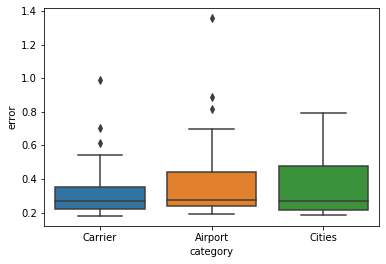
\includegraphics[width=0.6\textwidth, height=0.24\textheight]{./img/cats_arrdelay.png}
  \centering
  \caption{
  Distribución de errores promedio en predicción de delay de arribos (en minutos) sobre 4 splits de cross-validation para cada entidad del top5 de cada categoría.
  }
  \label{fig:cats-arrdelay}
\end{figure}

\begin{figure}[h]
  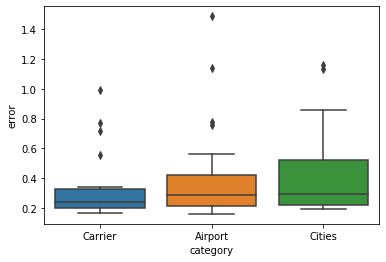
\includegraphics[width=0.6\textwidth, height=0.24\textheight]{./img/cats_depdelay.png}
  \centering
  \caption{
  Distribución de errores promedio en predicción de delay de partidas (en minutos) sobre 4 splits de cross-validation para cada entidad del top 5 de cada categoría.
}
  \label{fig:cats-depdelay}
\end{figure}
\subsubsection{El 9/11 y el impacto en predicciones de OTP}
%  que paso el 9/11 y como se esperaria que afecte, que medidas de seguridad
%   pudieron haber tomado
%  rangos que tomamos y que resultados dieron
Otra pregunta que nos hicimos fue cómo afectó, a través de la reacción en términos de políticas y rigor aeroportario, el atentado del 9/11 en Estados Unidos a las predicciones sobre delay. Consideramos por un lado que podría ser posible ver aumentos en delay por cuestiones de mayores exigencias de seguridad antes de salir a pista, o sino ver un decrecimiento en delays provocado por mayor planificación en respuesta, en ambos casos generando errores de predicción.

\begin{figure}[h]
  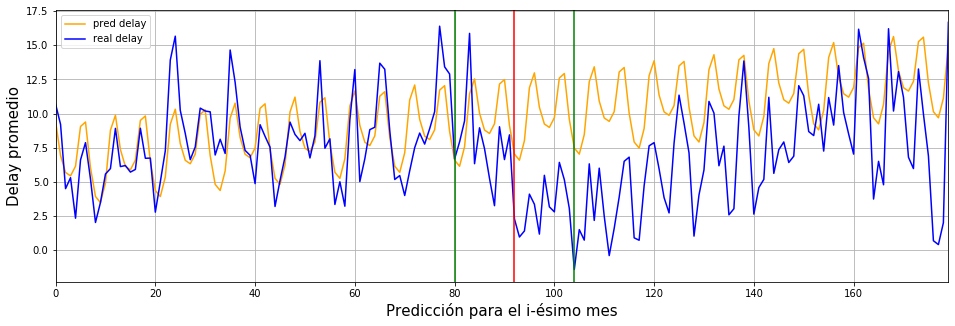
\includegraphics[width=1.0\textwidth, height=0.24\textheight]{./img/nine_eleven.png}
  \centering
  \caption{
  Predicción de delay en minutos contra delay histórico. Las líneas verdes marcan el intervalo de predicción sobre el cual se considera el error antes y despues del atentando, representado por la línea roja.
}
  \label{fig:nine_eleven}
\end{figure}

Para experimentar entrenamos al predictor de CML con datos anteriores a un año antes del atentado y comparamos el NMSE de las predicciones antes del atentado contra un año después del mencionado. En predicciones diarias notamos una diferencia entre aproximadamente 0.11 y 0.17 de RMSE antes y después del atentado respectivamente mientras que la diferencia en predicciones mensuales resultó de 0.28 y 1.26, con lo que resultaría que el impacto a nivel predicciones es importante (como se puede apreciar en la figura \ref{fig:nine_eleven}). Indagando más profundo descubrimos que el promedio de delay pasó de al rededor de 8 minutos antes del atentado a 3 luego de este, validando la hipótesis de una mayor planificación.
